
    \subsection*{A two-neuron network: starting backprop}
        
        Above, we mention "\textbf{each} layer": we'll now transition to a \textbf{two-neuron} system, so we have "two layers". Then, we'll build up to many layers.
        
        Remember, though, that the \textbf{ideas} represented here are just extensions of what we did \textbf{above}.
        
        Let's get a look at our \textbf{two-neuron} system, now with our \textbf{loss} unit:
        
        \begin{figure}[H]
            \centering
            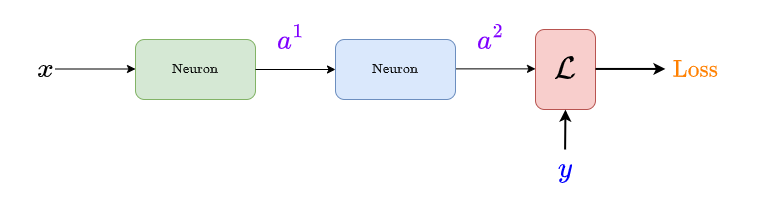
\includegraphics[width=140mm,scale=0.4]{images/nn_1_5_images/two_neurons_bp.png}
        \end{figure}
        
        And unpack it:
        
        \begin{figure}[H]
            \centering
            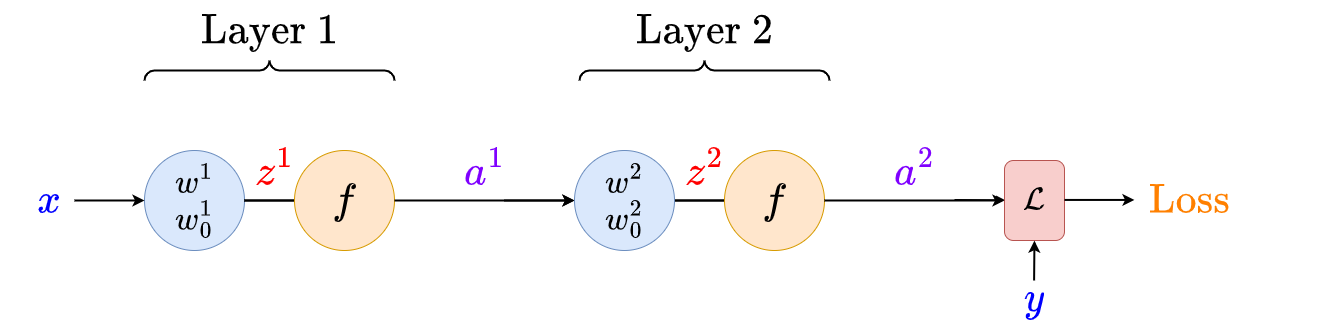
\includegraphics[width=140mm,scale=0.4]{images/nn_1_5_images/two_neurons_inside_bp.png}
        \end{figure}
        
        We want to do \textbf{back-propagation} like we did before. This time, we have \textbf{two} different layers of weights: $w^1$ and $w^2$. Does this cause any problems?
        
        It turns out, it doesn't! We mentioned in the first part of chapter 7 that we can treat the \textbf{output} of the \textbf{first} layer $a^1$ as the same as if it were an \textbf{input} $x$.
            \note{This is one of the biggest benefits of neural network layers!}
            
        \begin{figure}[H]
            \centering
            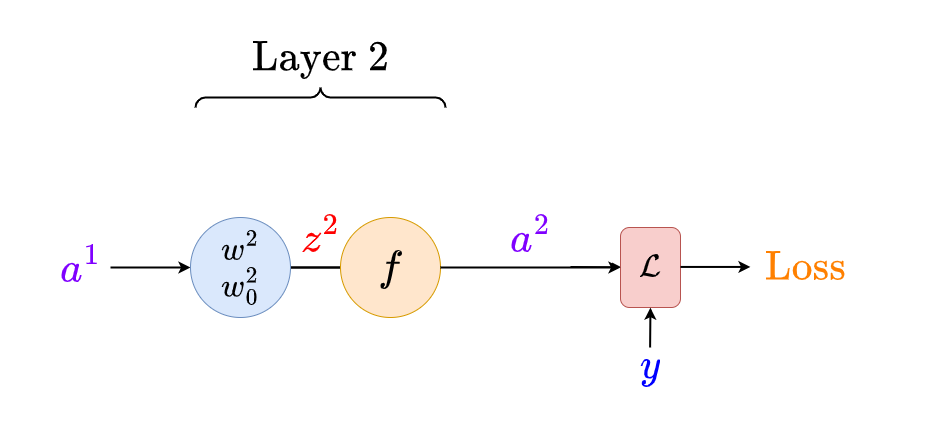
\includegraphics[width=90mm,scale=0.4]{images/nn_1_5_images/layer2_bp.png}
        \end{figure}
        
        Now, we can do backprop safely.
            \note{"Backprop" is a common shortening of "back-propagation".}
        
        \begin{figure}[H]
            \centering
            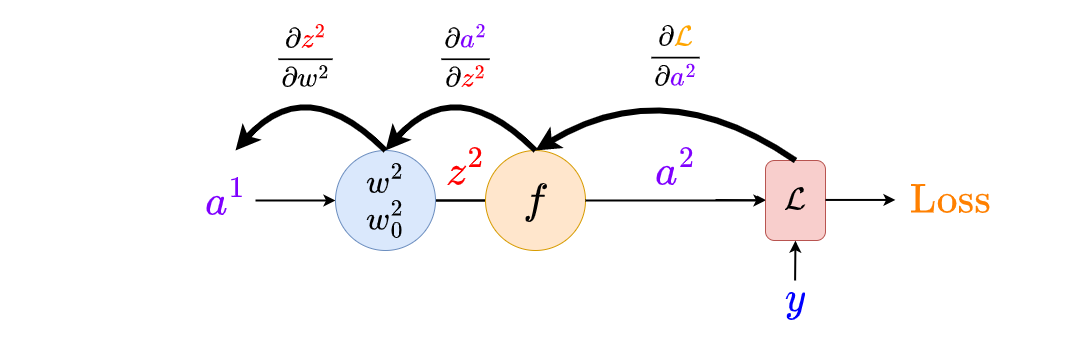
\includegraphics[width=120mm,scale=0.4]{images/nn_1_5_images/layer2_bp1.png}
        \end{figure}
        
        We can get:
        
        \begin{equation}
            \pderiv {\pur{\loss}} {w^2} 
            =
            \overbrace{
                \pderiv {\pur{\loss}} {\blu{a^2}} 
            }^{\text{Loss unit}}
            \cmul
            \overbrace{
                \pderiv {\blu{a^2}}     {\red{z^2}}
            }^{\text{Activation}}
                \cmul
            \overbrace{
                \pderiv {\red{z^2}}     {w^2}
            }^{\text{Linear}}
        \end{equation}
        
        The same format as for our \textbf{one-neuron} system! We now have a gradient we can update for our \textbf{second} weight vector.
        
        But what about our \textbf{first} weight vector?
        
    \secdiv
    
    \subsection*{Continuing backprop: One more problem}
    
        We need to continue further to reach our \textbf{earlier} weights: this is why we have to work \textbf{backward}.\\
        
        \begin{concept}
            We work \purp{backward} in \vocab{back-propagation} because every layer after the \gren{current} one \purp{affects} the gradient.
            
            Our current layer \gren{feeds} into the next layer, which feeds into the layer after that, and so on. So this layer affects \purp{every} later layer, which then affect the loss.
            
            So, to see the effect on the \purp{output}, we have to \gren{start} from the \purp{loss}, and get every layer \purp{between} it and our weight vector.
        \end{concept}
            
            \note{Remember that when we say "$f$ feeds into $g$", we mean that the output of $f$ is the input to $g$.}
            
        \phantom{ }
            
        \begin{figure}[H]
            \centering
            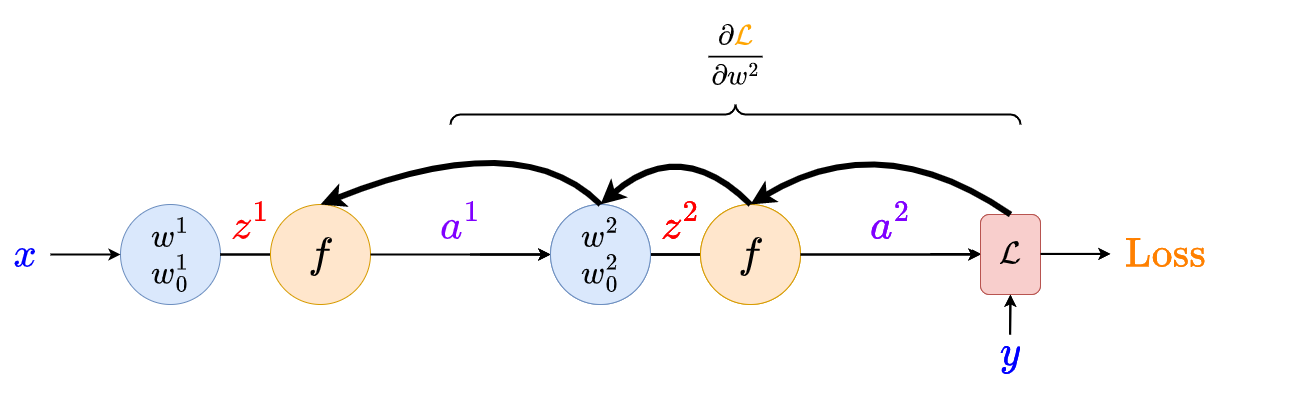
\includegraphics[width=120mm,scale=0.4]{images/nn_1_5_images/two_neurons_inside_bp2.png}
        \end{figure}
            
        We have one problem, though: 
        
        We just gathered the derivative $\pderivslash {\pur{\loss}} {w^2} $. If we wanted to continue the chain rule, we would expect to add more terms, like:
            \note{Since our current derivative includes $w^2$, we would continue it with a $w^2$ in the 
            "top" of a derivative, 
            $$\pderiv{\pur{\loss}}{w^2} \pderiv{w^2}{r}$$
            We're not sure what "$r$" is yet.}
        
        \begin{equation}
            \pderiv{w^2}{a^1}
        \end{equation}
        
        The problem is, what is $w^2$? It's a vector of constants.
        
        \begin{equation}
            w^2 = 
            \begin{bmatrix}
                    w_1^2 \\ w_2^2 \\ \vdots \\ w_n^2
            \end{bmatrix}
            ,
            \qquad
            \qquad
            \text{Not a function of $a^1$!}
        \end{equation}
        
        That derivative above is going to be \textbf{zero}! In other words, $w^2$ isn't really the \textbf{input} to $z^2$: it's a \textbf{parameter}.
            \note{We were building our chain rule by combining inputs with outputs: that's what links two layers together.\\
            \phantom{ }\\
            So, it should make sense that using something like $w$ (that doesn't link two layers) prevents us from making a longer chain rule.}
            
        So, we can't end our derivative with $w^2$. Instead, we have to use something else. $z^2$'s real input is $a^1$, so let's go directly to that!
        
        \begin{figure}[H]
            \centering
            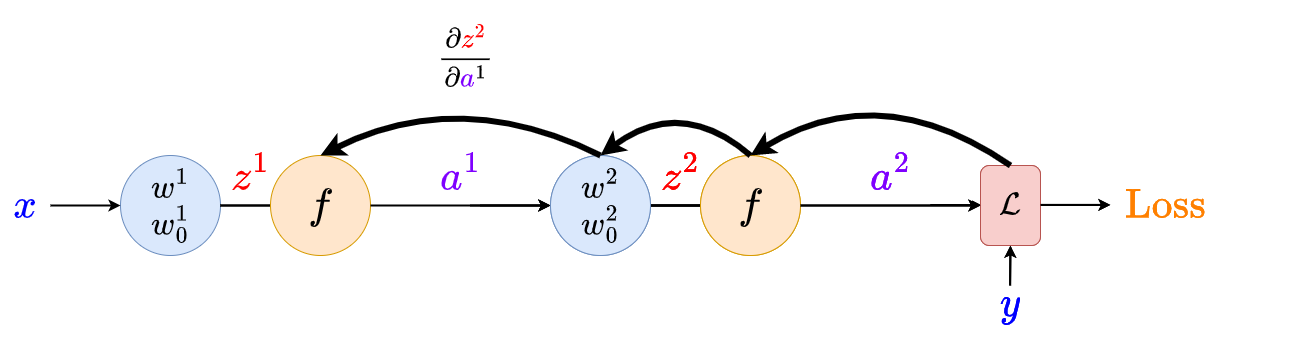
\includegraphics[width=120mm,scale=0.4]{images/nn_1_5_images/two_neurons_inside_bp3.png}
            \caption*{Using this allows us to move from layer 2 to layer 1.}
        \end{figure}
        
        Now, we have our new chain rule:
        
        \begin{equation}
            \pderiv {\pur{\loss}} {a^1} 
            =
            \overbrace{
                \pderiv {\pur{\loss}} {\blu{a^2}} 
                    \cmul
                \pderiv {\blu{a^2}}   {\red{z^2}}
            }^{\text{Other terms} } 
                \cmul
            \overbrace{
                \pderiv {\red{z^2}}   {a^1}
            }^{\text{Link Layers}}
        \end{equation}
        
        \begin{concept}
            For our \vocab{weight gradient} in layer $l$, we have to end our \purp{chain rule} with
            
            \begin{equation*}
                \pderiv {\red{z^\ell}}   {w^\ell}
            \end{equation*}
            
            So we can get 
            
            \begin{equation*}
                \pderiv {\pur{\loss}} {w^\ell} 
                =
                \overbrace{
                    \pderiv {\pur{\loss}} {\red{z^\ell}} 
                }^{\text{Other terms} }
                \cmul  
                \overbrace{
                    \pderiv {\red{z^\ell}}   {w^\ell}
                }^{\text{Get weight grad}}
            \end{equation*}
            
            However, because $w^l$ is not the \textbf{input} of layer $l$, we can't use it to find the gradient of \gren{earlier layers}.
            
            Instead, we use 
            
            \begin{equation}
                \pderiv {\red{z^\ell}}   {a^{\ell-1}}
            \end{equation}
            
            To "\purp{link together}" two different layers $\ell$ and $\ell-1$ in a \gren{chain rule}.
        \end{concept}
        
            \note{In this section, we compressed lots of derivatives into 
            $$\pderiv {\pur{\loss}} {\red{z^\ell}}$$
            Don't let this alarm you, this just hides our long chain of derivatives!}
            
    \secdiv
    
    \subsection*{Finishing two-neuron backprop}
    
        Now that we have safely connected our layers, we can do the rest of our gradient. First, let's lump together everything we did before:
        
        \begin{figure}[H]
            \centering
            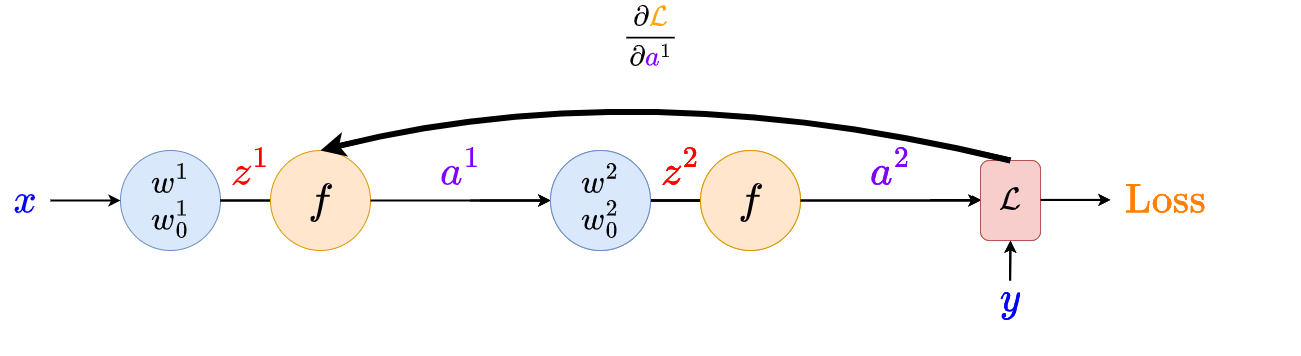
\includegraphics[width=120mm,scale=0.4]{images/nn_1_5_images/two_neurons_inside_bp4.png}
            \caption*{All the info we need is stored in this derivative: it can be written out using our friendly chain rule from earlier.}
        \end{figure}
        
        Now, we can add our remaining terms. It's the same as before: we want to look at the pre-activation
        
        \begin{figure}[H]
            \centering
            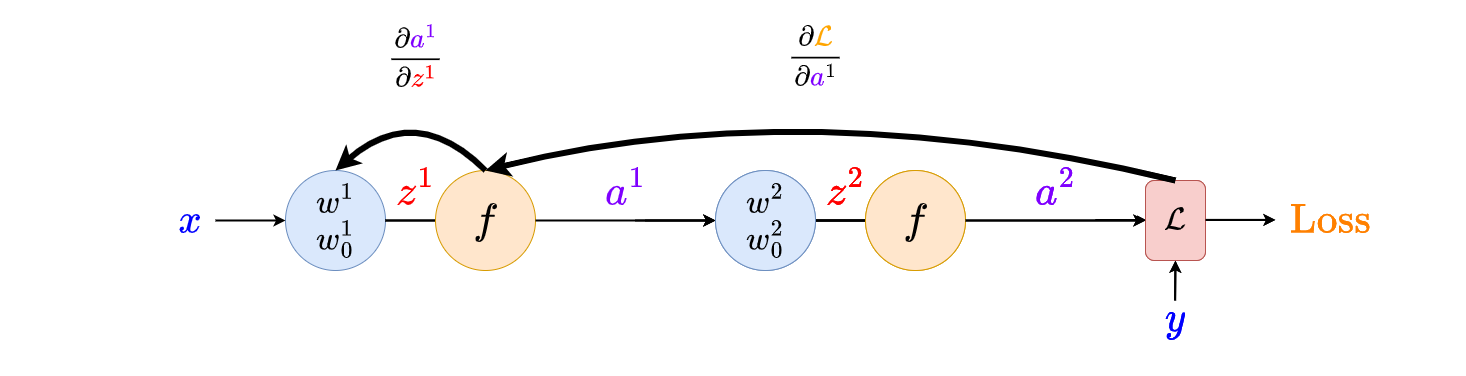
\includegraphics[width=120mm,scale=0.4]{images/nn_1_5_images/two_neurons_inside_bp5.png}
        \end{figure}
        
        And finally, our input:
        
        \begin{figure}[H]
            \centering
            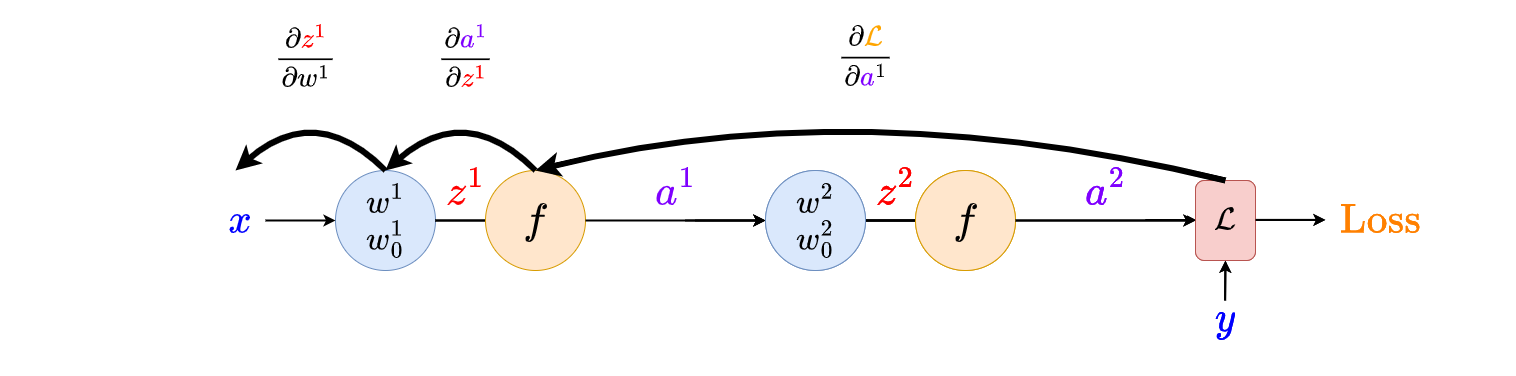
\includegraphics[width=120mm,scale=0.4]{images/nn_1_5_images/two_neurons_inside_bp6.png}
        \end{figure}
        
        We can get our second chain rule
        
        \begin{equation}
            \pderiv {\pur{\loss}} {w^1} 
            =
            \overbrace{
                \pderiv {\pur{\loss}} {\blu{a^1}} 
            }^{\text{Other layers}}
            \cmul
            \overbrace{
                \pderiv {\blu{a^1}}   {\red{z^1}}
                \cmul
                \pderiv {\red{z^1}}   {w^1}
            }^{\text{Layer 1}}
        \end{equation}
        
        Which, in reality, looks much bigger:
        
        \begin{equation}
            \pderiv {\pur{\loss}} {w^1} 
            =
            \overbrace{
                \Bigg(
                    \pderiv {\pur{\loss}} {\blu{a^2}} 
                \Bigg)
            }^{\text{Loss unit}}
            \cmul
            \overbrace{
                \Bigg(
                    \pderiv {\blu{a^2}}   {\red{z^2}}
                        \cmul
                    \pderiv {\red{z^2}}   {a^1}
                \Bigg) 
            }^{\text{Layer 2}}
            \cmul
            \overbrace{
                \Bigg(
                    \pderiv {\blu{a^1}}   {\red{z^1}}
                        \cmul
                    \pderiv {\red{z^1}}   {w^1}
                \Bigg)
            }^{\text{Layer 1}}
        \end{equation}
        
        We see a clear \textbf{pattern} here! In fact, this is the procedure we'll use for a neural network with \textbf{any} number of layers.\\
        
        \begin{concept}
            We can get all of our \vocab{weight gradients} by repeatedly appending to the \purp{chain rule}.
            
            For each layer, we multiply by
            
            \begin{equation*}
                \overbrace{
                    \pderiv {\blu{a^\ell}} {\red{z^\ell}}
                }^{\text{Within layer}}
                    \cmul
                \overbrace{
                    \pderiv {\red{z^\ell}} {w^\ell}
                }^{\text{Get weight grad}}
            \end{equation*}
            
            To get the \purp{weight gradient} $\pderivslash{ \pur{\loss} }{w^\ell}$.
            
            If we want to \gren{extend} to the next layer, we \red{instead} multiply by
            
            \begin{equation*}
                \overbrace{
                    \pderiv {\blu{a^\ell}} {\red{z^\ell}}
                }^{\text{Within layer}}
                    \cmul
                \overbrace{
                    \pderiv {\red{z^\ell}} {a^{\ell-1}}
                }^{\text{Link layers}}
            \end{equation*}
            
        \end{concept}
        